In the domain of drone systems, effective communication stands as a central pillar for operational success.
Communication with drones refers to the process of transmitting and receiving information between a drone and a remote control device or computer system. 
It involves the use of various technologies, including Wi-Fi, Bluetooth, and radio frequency (RF) signals, to control the drone and receive real-time data and feedback.

This chapter focuses on a crucial element of our drone programming environment: the Communication Framework. 
Its purpose is to handle all the communication between the ground station and the flying drone. 
More in detail, the Communication Framework is a software component hosted on the ground station 
that allows the user to establish effective communication between the script running on the ground station and the drone.

The Communication Framework manages the communication stream into two separate flows: parameter setting and telemetry logging.
The former is the flow of communication that is directed from the ground station to the drone; it is used to set configuration parameters onboard the drone.
The latter is the opposite flow of communication, from the drone to the ground station, and it is used to receive all the telemetry data of the drone, allowing for better control.


\section{The Communication Infrastructure}\label{sec:communication_infrastructure}
Before diving into the details of our Communication Framework, it is crucial to understand the underlying communication infrastructure. 

As described in Chapter~\ref{ch:tools}, our programming environment is spread into two main devices: the ground station and the drone.
The drone's firmware is written in C++ and runs on a small board with limited resources. On the other side, the ground station runs Python scripts
that control the drone's behavior. The heterogeneity between these two subsystems increases the complexity of the communication process.

The platform uses a custom network protocol called CRTP to overcome all these challenges. 
CRTP was designed to allow packet prioritization to help real-time control of the Crazyflie; in the current implementation, the link guarantees strict packet ordering within a port.

As shown in figure~\ref{fig:communication_stack}, the Crayzyflie communication is implemented as a stack of independent layers.
Every layer of the communication stack has two parallel implementations, one hosted in the firmware onboard and the other on the ground station's software.

The physical layer is responsible for transmitting packets to and from the Crazyflie. 

The link implements safe and ordered packet channels to and from the Crazyflie. This layer abstracts the physical medium and implements one transmitting and receiving packet channel to and from the Crazyflie.

The CRTP layer introduces the concept of a logical packet; each packet measures 32 Bytes and is composed of three parts: port, channel, and payload.
The tuple \textit{port:channel} allows the packet to be delivered to the specialized subsystem that receives and processes the message.

\sidecaptionvpos{figure}{c}
\begin{SCfigure}[\sidecaptionrelwidth][h]
    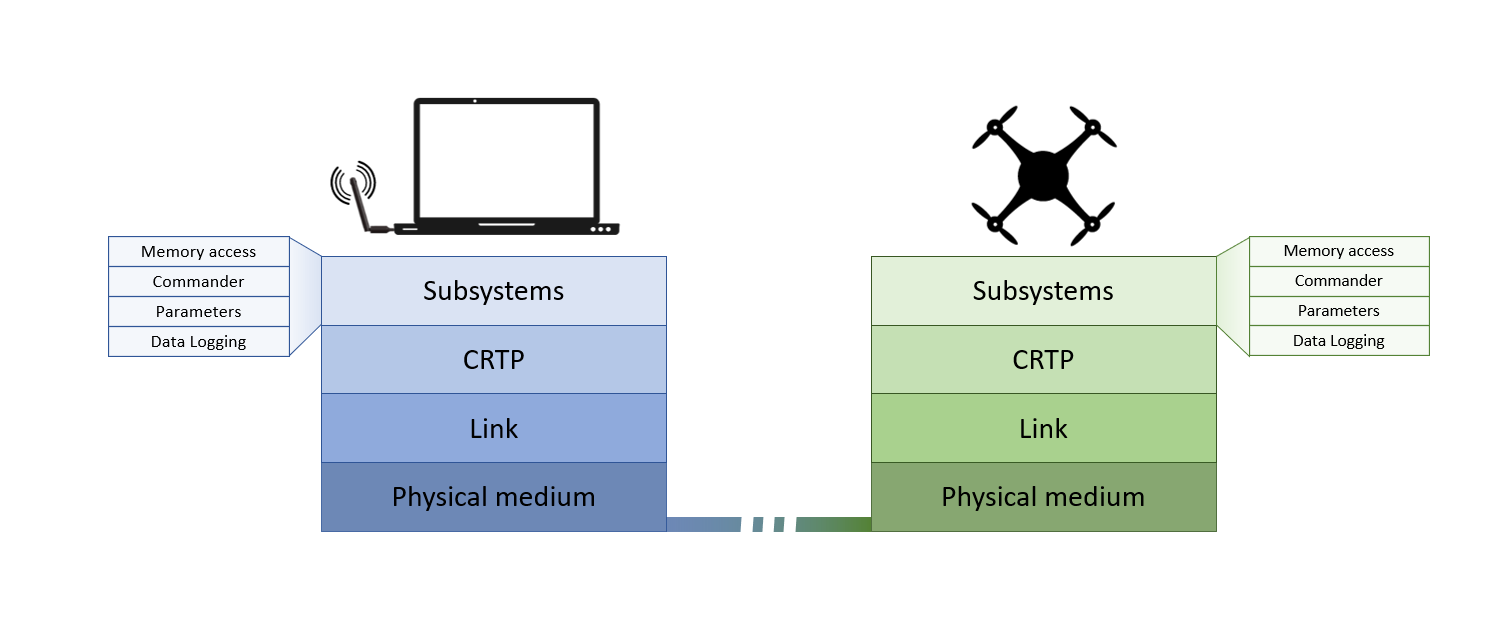
\includegraphics[width=0.5\textwidth]{communication/communication_stack}
    \caption[The Crazyflie communication stack]{The Crayzyflie communication stack is composed of 4 independent layers: Subsystems, CRTP, Link, Physical medium}
    \label{fig:communication_stack}
\end{SCfigure}

In the higher-order layer, we can identify four principal subsystems:
\begin{itemize}
    \item \textbf{Memory access} -- that manages memory operation on the Crazyflie's physical memories, e.g., trajectory uploading.
    \item \textbf{Commander} -- that send/receive control set-points.
    \item \textbf{Parameters} -- that manages read/write operations on configuration parameters of the Crazyflie.
    \item \textbf{Data Logging} -- that handles logs of telemetry data sent periodically from the Crazyflie to the ground station. 
\end{itemize} 

The first two subsystems (memory access and commander) are the simplest, with a straightforward implementation. 
They expose some methods through an API, and when called, they craft a packet, fill it with parameters data, and send it to the link layer.
On the other side, the same subsystem receives the packet, unpacks the data, and executes the desired function.

Conversely, the parameters and data logging subsystems have some peculiarities that make them more complex. 
In particular, the parameters subsystem allows performing read/write operations with acknowledgments of the successful operation.
The data logging subsystem, instead, must support periodical updates of telemetry data.
Moreover, both the two subsystems must handle a variety of variables with different types.

The Communication Framework that we designed and developed is meant to wrap the functionalities of these two complex subsystems and offer the user a more usable and efficient way to handle data logging and parameters.


\section{The Design of the Communication Framework}\label{sec:communication_frameworks_design}

The Communication Framework is a software component that provides an easy and accessible way to set parameters onboard the Crazyflie and to log telemetry data.
This component is part of the ground station's software and has been designed as a publish/subscribe system.

Every CRTP data that is routed to the parameter or logging subsystem is managed by the Communication Framework and stored in a central repository.
Every other software component or script interested in such data can use the Communication Framework to access the repository and subscribe for value updates.

Given the profound semantic difference between the logging and parameters subsystems, we decided to keep the two concepts separated inside the Communication Framework.
For this reason, we developed two different Communication Managers, one for every subsystem. The two implementations, namely the Logging and the Parameters Manager, 
shares the publish/subscribe design structure, but they slightly differ in the management of the updates in the repository.

\subsection{The Logging Manager}\label{subsec:logging_manager}

As described above, the Logging Manager is one of the two implementations of the Communication Framework. 
In particular, the role of the Logging Manager is to handle the setup and the periodic updates of telemetry data sent from the Crayzyflie.

The internal structure of this component is represented by a values repository where key-value pairs are stored to maintain the telemetry state.
More in detail, each variable, identified by a unique key, represents an entry inside the values repository; the value of the entry is the last updated value of the logged variable.

In a separate repository, the Logging Manager stores the subscribers interested in the variables updates. 
In this second repository, the component stores a list of references to subscribers for each single variable or set of variables. 
Each reference consists of a predicate function to allow filtering updates and a callback function to effectively notify the subscriber when the predicate is satisfied with the new value.

To better understand the working principle behind the Logging Manager, we illustrated the complete workflow in Figure~\ref{fig:logging_manager}.

Whenever the script running on the ground stations needs to start tracking a variable, the Logging Manager creates or updates a log configuration and sends it to the Crazyflie.
The configuration contains information regarding the variable name, the type, and the desired period of updates. 

At some point, when the script is interested in reading and getting updated on the variable's values, it creates a callback function, i.e., an action to be executed with the new updated value, and, optionally, a predicate function for receiving updates only when the values satisfy certain constraints.

Then, the script registers these functions to the Logging Manager, specifying the single variable or set of variables of interest.
When the logging process starts, the Crazyflie sends periodic messages containing the variable updates; the Logging Manager intercepts those messages and updates its internal values repository.
Each time an update occurs, the Logging Manager checks whether any subscriber is watching that variable. 
If so, for each subscriber, it evaluates the predicate and eventually notifies the subscriber by calling the registered callback. 

\begin{figure}[h]
    \centering
    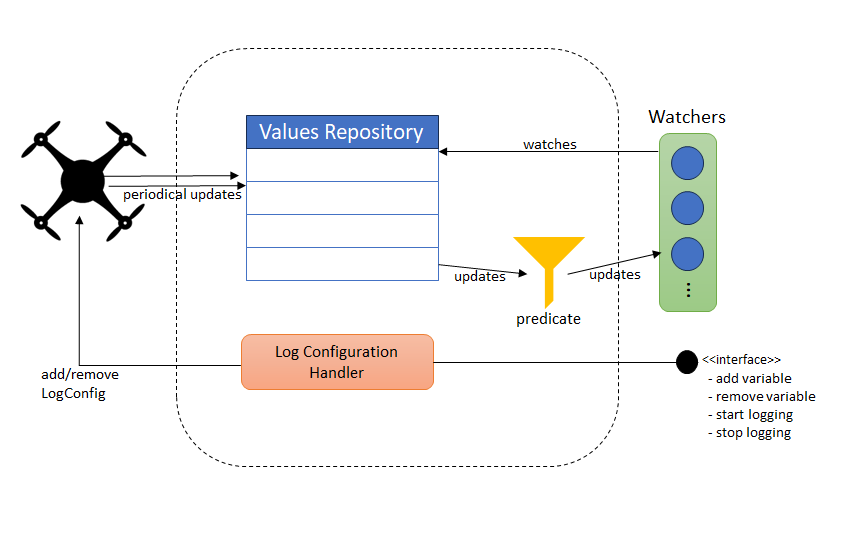
\includegraphics[width=0.9\textwidth]{communication/logging_manager}
    \caption{Logging Manager's workflows.}\label{fig:logging_manager}
\end{figure}

Given that each variable can have its own size (given the type) and period, the Logging Manager needs to handle different log configurations.
Moreover, the single configuration has a size constraint of 26 Bytes given by the size of the CRTP packet, increasing the complexity of the configuration management.

To optimize the number of log configurations created, each time the Logging Manager needs to add a variable, 
it searches for a suitable existing configuration with enough space to fit it. 
The Logging Manager only adds a new configuration when strictly necessary, ensuring maximum optimization.

\subsection{The Parameters Manager}\label{subsec:parameter_manager}

The other implementation of the Communication Framework, the Parameters Manager, manages the configuration operations of the Crayzyflie.
The Crayzyflie 2.1 allows the users to set parameter values to configure the desired setup. 
An example of a parameter could be the selected state estimator, i.e., Extended Kalman Filter or Complementary Filter (See Section~\ref{sec:state_estimate_and_control}).

Following the same structure as the Logging Manager, also the Parameters Manager has one value and one subscriber repository where it stores, respectively, the current value for tracked parameters and the references of subscrbers for each variable.

Conversely, variable updates are managed slightly differently with respect to the Logging Manager. 
In fact, the underlying parameters subsystem does not have a periodic update of values; instead, the updates happen only when the parameter's value is effectively changed onboard.
In other words, the Parameters Manager only receives and processes an update when the Crazyflie acknowledges a state change in the parameter's value.
 
Figure~\ref{fig:parameters_manager} represents the operations workflow inside the Parameters Manager. When needed, usually before the takeoff,
the script can use the Parameters Manager to read or write configuration values. 

Read operations are processed straightforwardly with a synchronous request-response messages exchange. 
The request contains the name of the variable, and the Crazyflie's response contains the current value of the requested parameter.

Write operations, on the other side, are processed asynchronously; first, a request message is sent from the Parameters Manager to the Crazyflie,
then, when the Crayzyflie successfully completes the update, it notifies the ground station's Parameters Manager.

Once the Parameters Manager receives a value, it uses the internal publish/subscribe system to notify subscribers.  

\begin{figure}[h]
    \centering
    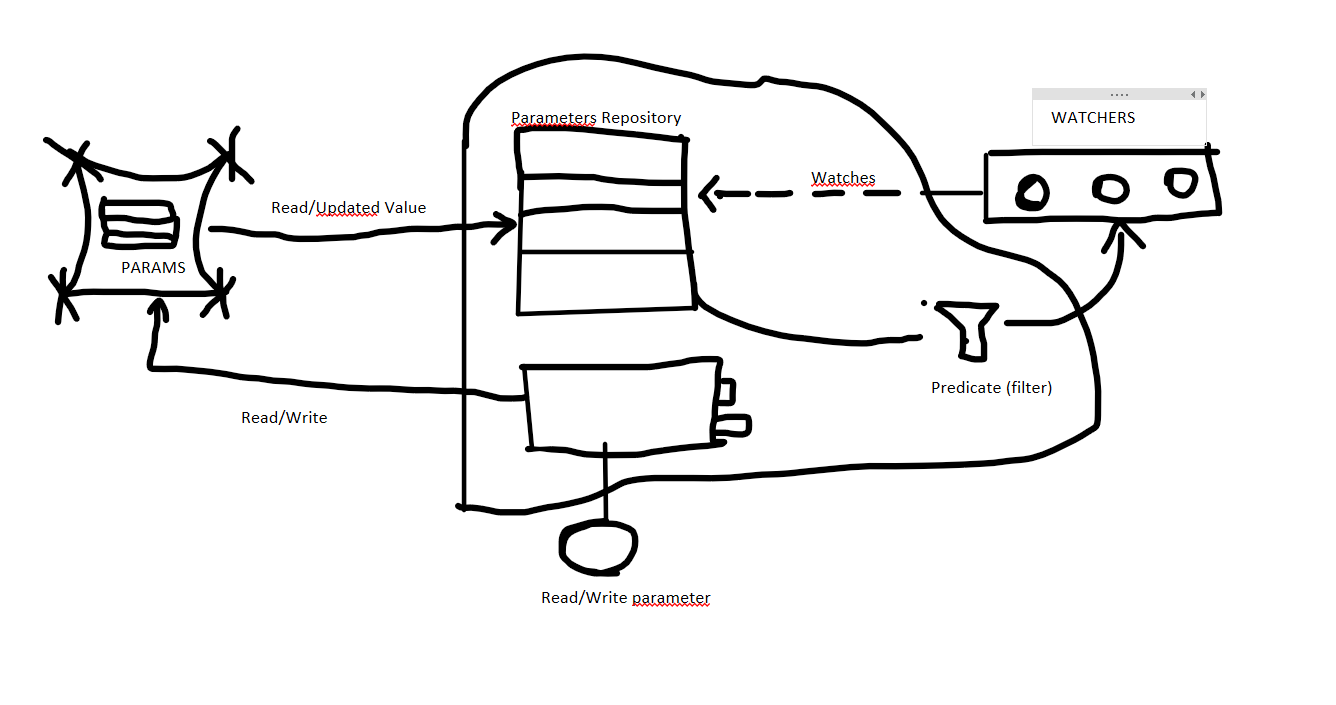
\includegraphics[width=0.9\textwidth]{communication/parameters_manager}
    \caption{Parameters Manager's workflows.}\label{fig:parameters_manager}
\end{figure}

